\chapter{AppShield系统}
\label{chap:appshield}

本文对大规模应用审查系统进行了设计,并实现了原型系统AppShield。
本章将对AppShield系统进行详细的介绍。
在~\ref{sec:appshield:overview}节中,我们对AppShield的工作流程进行了简单介绍;
在~\ref{sec:appshield:collection}节中,我们将介绍了AppShield中应用文件收集的两个方式;
在~\ref{sec:appshield:file-analyze}节中,我们介绍了AppShield中使用的文件分析器Apkinsight;
而AppShield的核心,问题组件分析以及相似度分析将分别在~\ref{sec:appshield:comp-analysis}节和~\ref{sec:appshield:sim-analysis}中介绍。
最后在~\ref{sec:appshield:conclusion}节中,我们将对本章内容进行小结。

\section{AppShield工作流程}
\label{sec:appshield:overview}

AppShield系统主要分为两个部分,采集部分主要目的是持续获取APK文件,分析部分目标是在搜集到的APK里自动找到有隐私问题的应用,自动总结隐私泄露的规律,并且对有问题组件进行进一步的分析。
同时AppShield还会基于相似度检测的方法对应用进行第三方检测以及克隆应用检测。
如图~\ref{fig:appshield-overview}所示,AppShield采集部分通过两种方式获取安卓应用APK文件,一方面系统有一个长期运行的爬虫程序,从多个应用市场获取最新的应用,另一方面AppShield通过合作的形式,从appaudit.io获得样本进行分析。
appaudit.io允许用户上传应用并使用AppAudit进行分析,并将检测结果呈现给用户,AppShield可以从appaudit.io后台获取用户提交的应用APK文件,收集到的APK文件存入AppShield的文件数据库中。
同时,从市场或者用户方面获得的APK文件的元数据(例如下载量、文件名等等)也将自动进入数据库。

\begin{figure}
	\centering
	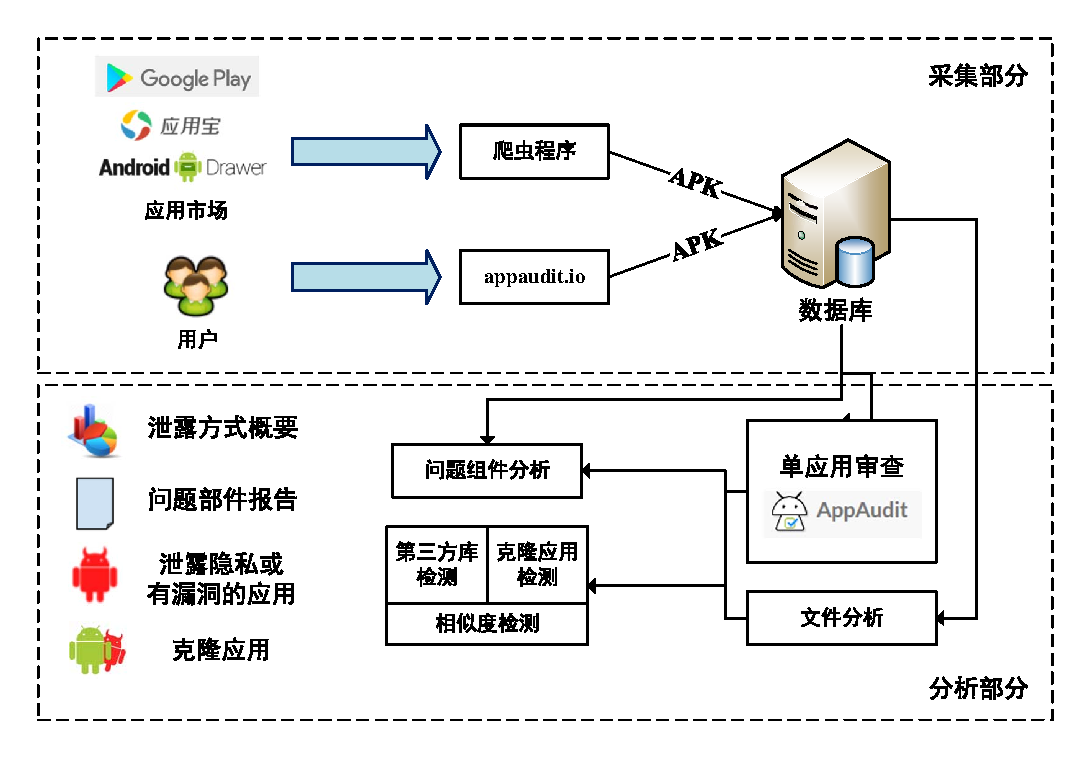
\includegraphics[width=0.8\textwidth]{figure/appshield-overview.pdf}
	\bicaption[fig:appshield-overview]{AppShield系统架构图}{AppShield系统架构图}{Fig}{Overview Architecture of AppShield}
\end{figure}


AppShield分析部分开始先对数据库中每个APK进行文件分析,提取APK文件中提取App信息(例如应用的名称、识别名、版本、代码中每一个类名等等),放入数据库。
然后(并行地)由AppAudit进行的单App隐私审查,标志出每个App中可以识别的隐私问题。
文件以及AppAudit分析的结果会被用于启动“问题组件分析”,用于找到应用中造成隐私问题的组件,并确认其版本,输出统计结果、问题组件的报告(包括关键样本等)。
另外AppShield提出了一种基于指纹的相似度检测方法,该方法可以应用与第三方库检测和克隆应用检测中。
AppShield会利用此方法对应用进行第三方库和克隆应用检测,最终检测出具有隐私问题或漏洞的应用以及克隆应用。

AppShield系统选择MongoDB作为数据库储存应用元数据。
首先,MongoDB自身拥有性能优秀、可靠性高、社区支持良好的有点。
其次,更重要的是,AppShield系统中的数据交换都使用JSON格式;
JSON格式不仅易于人类阅读和编写,也十分适合机器解析和生成,被广泛接受和使用。
而MongoDB中的数据以BSON(一种JSON的二进制表达和扩展)储存,所以JSON格式与MongoDB天然地相适应。
AppShield系统将应用APK文件储存在共享文件系统而不是数据库中。
每个APK文件有相应的SHA1值,方便查找和去重,并且优化APK在真实文件系统上的存储(文件名统一长度,目录层次完整)。

\section{应用文件收集}
\label{sec:appshield:collection}

应用文件主要来自于两个方面:爬虫程序和appaudit.io网站用户上传。

\subsection{爬虫程序}

AppShield系统的爬虫程序会不断从各个应用市场抓取应用的网页数据信息和APK文件,分别存储在数据库和共享文件系统中。
目前爬取的应用市场覆盖国内外的知名Android应用市场,详细情况见测试与评估部分的测试集。

在设计和实现爬虫程序时,有以下的要求以及实现考虑:
\begin{enumerate}
	\item 全自动的:
		给与一个或多个初始链接,爬虫程序能根据当前网页信息不断地生成下一个目标链接,最终能尽量覆盖整个应用市场。
	\item 同一应用的不同版本:
		在应用发布新版本后,爬虫程序要能及时将新版本的网页信息和APK文件抓取下来。
		在实现中,我们的爬虫会不断地重复扫描应用市场,根据网页上的应用发布日期、应用版本等信息,判断是否发生版本更新,并将新版网页数据和APK文件抓取下来。
		这样,我们就将一个应用几乎所有的版本保存在我们的数据库中。
	\item 容错性:
		爬取一个应用可能持续几分钟的时间(取决于当前网络状况和目标文件大小),而中途可能发生错误和故障,包括网络中断、网页出现404、爬虫程序被意外中止等。
		在实现中,我们将“爬取一个应用”视为一个事务,将“APK文件写入磁盘和网页数据写入数据库”作为这个事务的提交标志。
		通过这种方式,爬虫程序保证原子性和一致性:当错误发生后,已提交事务一定正确完成,未提交事务在未来再次遇到时会被重做。
	\item 并行性:
		应用市场的应用数量非常多,单线程爬虫无法有效地下载大量的应用。
		爬取不同应用本质来说是相互独立的,利用之前提到的基于消息队列的任务调度,爬虫程序很容易实现良好的并行性。
		除此以外,在实现中,利用上述的事务机制,我们保证同一个应用的同一个版本只会被成功提交一次。
\end{enumerate}


结合上述需求,我们以腾讯应用宝上微信应用的抓取为例,介绍一下爬虫的工作流程。
首先,爬虫程序会从腾讯应用宝获取各个分类下的热门免费应用列表,将它们作为初始链接加入爬虫程序的任务队列。
如图~\ref{fig:myapp-pop}所示,这是全部软件分类下的热门免费应用列表,列表中的微信会被作为初始链接添加进任务队列。
随后某个爬虫实例从任务队列中接受这个微信抓取任务,这时可以看作一个事务的开始。
爬虫实例先获取微信应用的HTML文档,如图~\ref{fig:wechat-detail}所示,页面包含大量有用的原始数据,例如评分、评论、下载量等等。
爬虫程序通过CSS选择器和DOM操作,准确定位这些元素,提取其中文本作为原始数据。
这时,爬虫程序会根据这些原始数据判断应用是否为免费应用、应用版本是否还未爬取过(是否有版本更新)。
通过这些判断后,爬虫程序开始下载APK文件。
下载完成后,再次确认APK文件没有重复,并将APK文件储存在共享文件系统中。
最后,网页原始数据被写入数据库,意味着这个微信抓取事务的提交。
如果之前任意一步出错,由于数据库中没有微信的原始数据,下一次遇到微信任务都会重新开始。
另外,页面中还包括了微信的相似应用链接和同开发者应用链接,这些链接会作为新的任务加入爬虫队列,加之初始链接来自于不同种类,保证了爬虫自动覆盖整个市场。

值得注意的是,对于Google Play,我们不能从网页上获取到应用APK文件的URL,因而我们无法简单地直接下载应用APK文件。
幸运的是,许多开发者都为Google Play提供了非官方API和下载模块。
在本系统中,我们使用 Akdeniz 开发的google-play-crawler,作为Google Play的下载器。它对非官方API进一步封装,我们只需提供应用的包名,它便开始查询并下载应用。

\begin{figure}
	\centering
	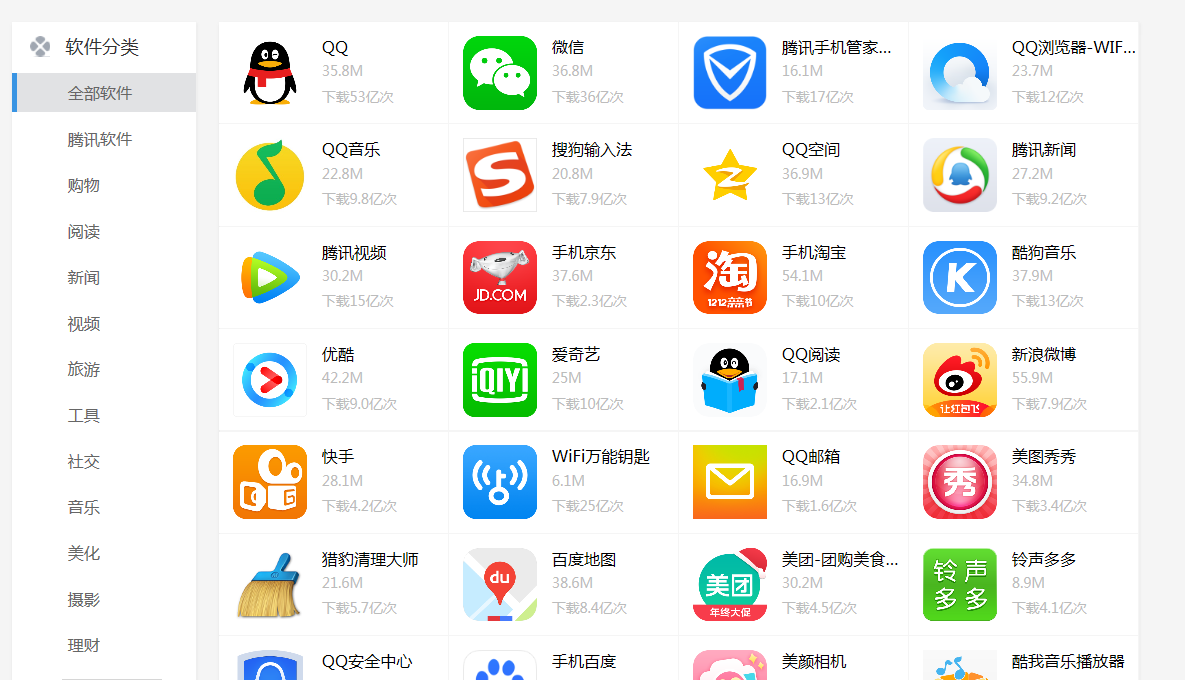
\includegraphics[width=0.8\textwidth]{figure/myapp-popular.png}
	\bicaption[fig:myapp-pop]{腾讯应用宝热门应用页面}{腾讯应用宝热门应用页面}{Fig}{Most Popular Apps in Tencent Myapp}
\end{figure}

\begin{figure}
	\centering
	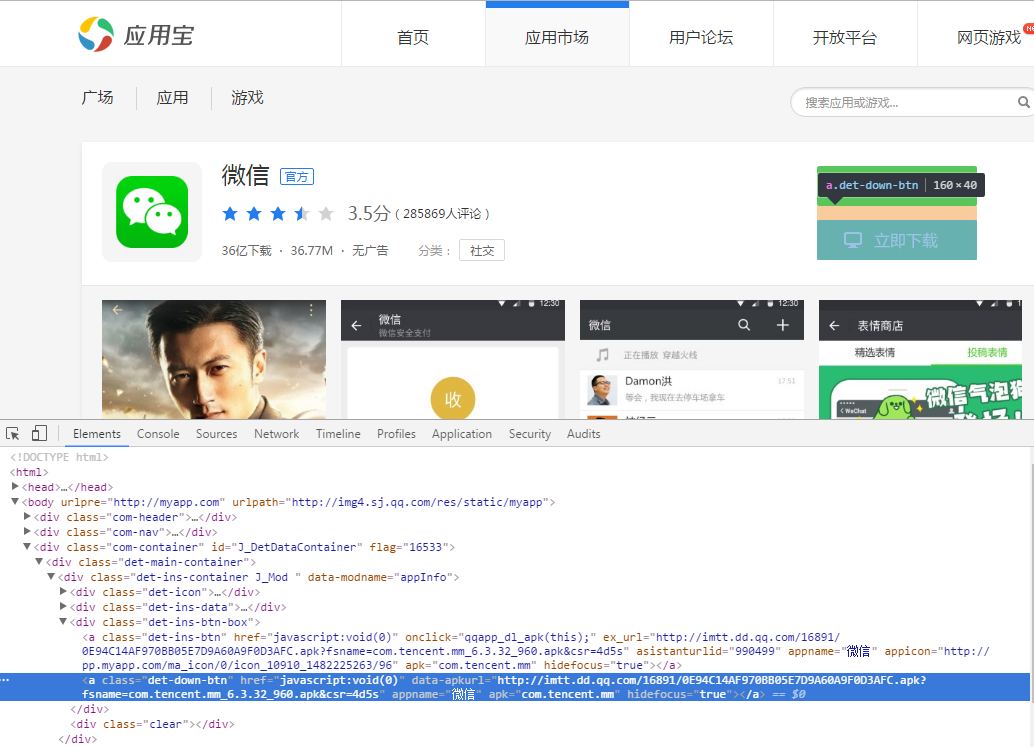
\includegraphics[width=0.8\textwidth]{figure/wechat-detail.png}
	\bicaption[fig:wechat-detail]{微信在应用宝中的详细页面以及下载链接}{微信在应用宝中的详细页面以及下载链接}{Fig}{Detail Info Page of Wechat in Myapp}
\end{figure}


\subsection{appaudit.io用户上传}

appaudit.io网站为用户提供了使用AppAudit的网站接口。
网站访问者可以上传APK文件进行审查,审查之后,网站会显示应用的检测结果。
检测结果包含了应用的基本信息,如应用名、报名、版本、Google Play评分以及应用的隐私泄露行为情况和危险权限使用情况。
图~\ref{fig:appaudit-sample}为appauditio检测出用户提交程序有恶意行为。

\begin{figure}
	\centering
	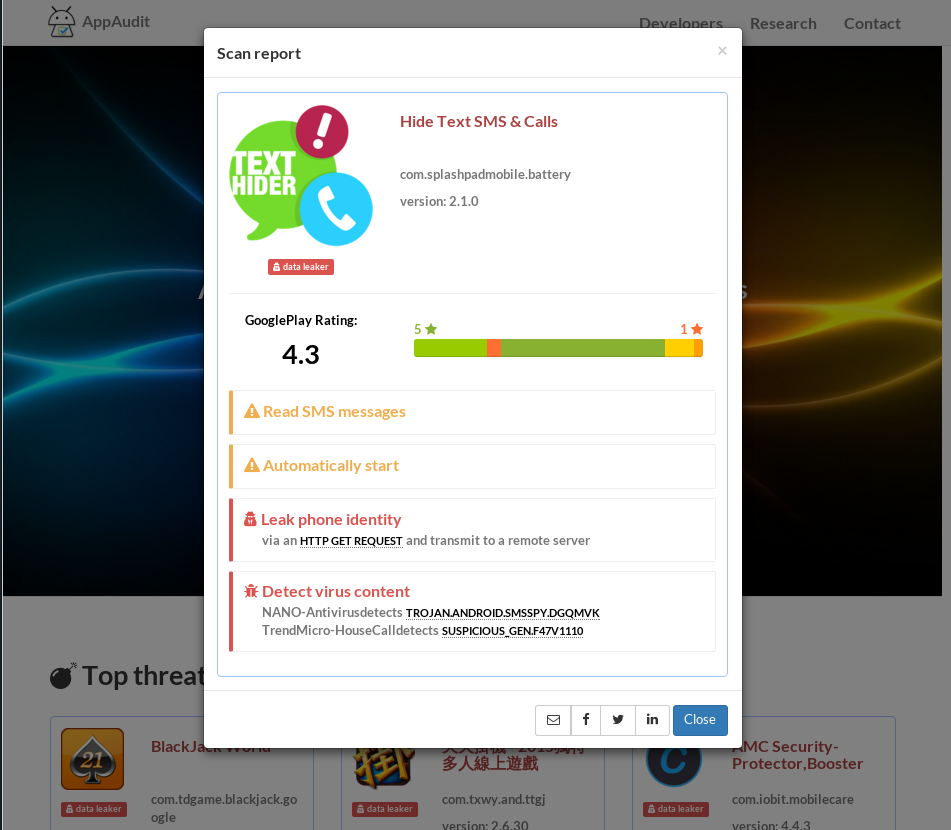
\includegraphics[width=0.8\textwidth]{figure/appaudit-sample.png}
	\bicaption[fig:appaudit-sample]{微信在应用宝中的详细页面以及下载链接}{微信在应用宝中的详细页面以及下载链接}{Fig}{Detail Info Page of Wechat in Myapp}
\end{figure}

\section{文件分析}
\label{sec:appshield:file-analyze}

在AppShield系统中,由于多个过程都需要对应用SDK进行分解并解析元数据,所以我们开发了Apkinsight文件分析器。
Apkinsight会对数据库中的APK文件进行初步分析,然后将提取整理后的APK元数据以规范的JSON格式输出并储存在数据库中。
Apkinsight分析提取的应用信息如表~\ref{tab:apkinsight}所示。


\begin{table}
	\centering
	\bicaption[tab:apkinsight]{Apkinsight文件分析器分析结果}{Apkinsight文件分析器分析结果}{Table}{Analysis Result of File Analyzer Apkinsight}
	\begin{tabularx}{\textwidth}{|c|c|X|}
		\hline
		提取信息分类 & 提取的信息 & 样例数据\\
		\hline
		应用基本信息 & 包名 & ["\texttt{com.tencent.mm}"]\\
		& 版本名 & \texttt{6.1.0.66\_r1062275}\\
		& 版本号 & 542\\
		& 安装包大小 & 21 MB\\
		& 权限列表 & ["\texttt{com.tencent.mm.permission.READ}"]\\
		& 安装位置 & /data/qq.apk\\
		\hline
		应用证书信息 & 开发者公钥及公钥指纹信息 & ...\\
		& 证书签名是否通过验证 & True\\
		\hline
		应用代码信息 & 代码是否混淆 & True\\
		& 类名列表 & ["\texttt{com.example.MainAcitivity}"]\\
		\hline
		应用内文件信息 & 文件路径 & res/1.jpg\\
		& 文件类型 & jpeg\\
		& 文件大小 & 14KB\\
		\hline
	\end{tabularx}
\end{table}


Apkinsight利用并整合了多种现有的工具,其中包括apktool、JDK中的keytool、jarsigner、baksmali等等。
APK是Android系统使用的应用包格式。
在Android应用构建时,首先应用代码会被编译成Java字节码,之后于Android框架jar包、类库jar包合并打包成classes.jar。
然后Dalvik编译器dx会把jar编译成Dalvik的字节码classes.dex。
然后apk打包器会将应用所用的资源以及Android描述文件AndroidManifest.xml进行二进制化,最后与dex代码、本地库等文件一起打包压缩成APK格式。
值得注意的是,此时生成的APK是未经过开发者签名的APK。
根据Android文档,只有经过签名的应用才能被安装\footnote{App Signing: \url{https://developer.android.com/studio/publish/app-signing.html}}。
对于一个Android应用开发者,需要为自己的应用生成一对公/私钥。
在对应用进行签署的过程会在META-INFO文件夹中生成三个文件MANIFEST.MF、CERT.SF、CERT.RSA。

其中MANIFEST.MF是应用的摘要文件,是利用SHA1对所有非文件夹非签名文件的文件进行哈希,然后通过BASE64进行编码。
这是一个简单的完整性验证,如果攻击者简单修改了程序而未修改此摘要信息,则在安装时会被发现,从而禁止安装。

CERT.SF是应用对摘要的签名,在签署过程中,会使用应用开发者的私钥对之前生成的MANIFEST.MF进行签名,此签名可以用私钥对应的公钥进行验证,从而验证应用开发者的身份。
所以即使攻击者在修改了程序代码的同时重新生成MANIFEST.MF,也无法经过此步的验证。

CERT.RSA中保存了应用开发者的公钥,在应用被安装时,系统会解析出应用的公钥,对CERT.SF进行验证,来验证应用开发者的身份,从而保证用户手机的安全。

Apkinsight的设计动机之一便是在于现有工具过于零散,例如对于应用证书的采集分析,我们会用到keytool、jarsigner、openssl等多个程序。
面对数量巨大的应用以及纷繁复杂的分析工具,研究者需要面对“使用何种工具”以及“如何使用”的困扰,无法专注于应用信息的处理。
Apkinsight对这些工具进行整合封装,为研究者提供统一的工具抽象,提供应用的基本元数据。

在Apkinsight中,会先使用apktool对apk进行解压并且对二进制化的资源文件进行反序列化,之后会使用baksmali将apk的dex代码文件反编译成smali格式以便之后更深度的分析。
同时Apkinsight会利用keytool、openssl以及jarsigner提取出应用的公钥以及公钥指纹信息,并且对应用的签名进行验证。
之后Apkinsight会解析应用的AndroidManifest.xml获取应用的元信息,并且对应用内文件进行遍历,进行信息收集。
最终会将Apkinsight提取整合过的元数据以规范的JSON格式储存在数据库中。
目前,应用元数据没有一种统一的定义与格式,为分析工作带来许多不便。
Apkinsight通过统一元数据格式,为之后的分析工作提供格式化信息

值得注意的是,Apkinsight提供了检测代码是否经过混淆的功能,是通过检测应用的本身包中是否包含Android资源类R来判断应用是否被混淆,关于判断的详细过程,会在~\ref{sec:appshield:proguard}节中进行详细介绍。

\section{问题组件分析}
\label{sec:appshield:comp-analysis}

Android应用数以亿计,质量参差不齐,其中也不乏有很多伪装成正常应用的病毒。
在正常应用中也可能包含各种各样的漏洞。
这些问题应用的源头往往存在于一个组件中,我们称这样的组件为问题组件。
一个组件是由一个包及其所有子包组成,一个存在安全漏洞的第三方库、一个泄露隐私的广告库或者一个伪装成正常包的病毒都是一个问题组件。
问题组件的来源可以有很多地方。
AppShield使用的单应用审查工具AppAudit的审查结果、第三方库的漏洞声明、病毒库都可以成为问题组件的来源。
在应用市场中,这样的问题包可能存在于很多应用中,当我们发现一个问题组件后,如何找出问题组件的“感染”应用,是在本节需要解决的问题。

我们在应用收集阶段,一共获得了116672个应用,其中37095是被检测出混淆的,占总体的31.8\%。
可见未混淆应用占了大部分比例,但是混淆应用也不能忽略不计。
所以针对混淆应用和未混淆应用,AppShield有着不同的处理方法。
对于未混淆应用,我们可以利用文件名、代码等信息来对问题组件进行识别,并对问题组件进行分析。
而对于混淆应用,这些信息都有可能在混淆过程中发生改变,所以需要设计更加稳定的方法来对问题组件进行检测。
对于混淆应用的处理方法,我们会在下一节中介绍。


\begin{figure}
	\centering
	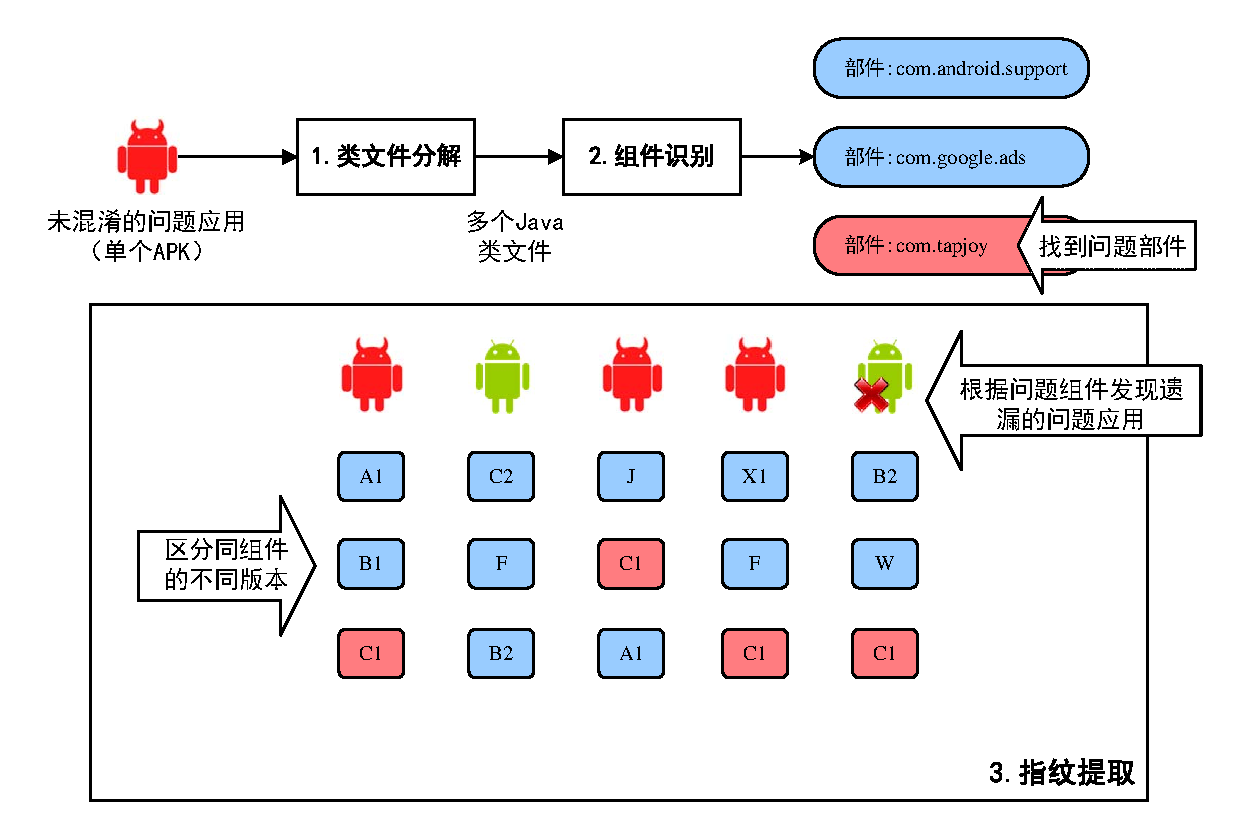
\includegraphics[width=0.9\textwidth]{figure/comp-analysis.pdf}
	\bicaption[fig:comp-analysis]{问题组件分析主要分析过程}{问题组件分析主要分析过程}{Fig}{Analysis Process of Problematic Components}
\end{figure}


如图~\ref{fig:comp-analysis}所示,在问题组件以及比对应用都未被混淆的情况下,AppShield的问题组件识别会进行以下三个步骤:

\begin{enumerate}
	\item 类文件分解:
		一个应用程序的代码将会按照Java类进行更细粒度的分割,每一个Java类文件中包含代码以及类的成员函数以及变量。
		分解后,每一个类文件或者来源自第三方组件,或者由应用开发者编写。
		所以分解后可以开始识别APK文件中用到了哪些第三方组件。
	\item 组件识别:
		被分开的Java类文件会进一步聚类,按照包结构将多个类组成一个组件,而识别出的组件会结合AppAudit的分析结果,将具有隐私问题的组件标记出来并将这些信息写入数据库。
	\item 指纹提取:
		用于区分同一个组件的不同一个版本,从而能够更准确确定哪个组件的哪个具体版本会造成隐私泄露。
\end{enumerate}

\subsection{类文件分解}
Android应用是用Java进行开发的,每个Java类源代码会逐一编译,然后合并到一个DEX文件中。
DEX是Android的可执行代码格式,包含Java字节码格式以及类的信息(函数原型、变量、行号等等)。
AppShield会首先解开DEX文件,将其分解为原来的一个个类文件,这是因为如果一个应用包含了某个第三方的组件,组件可能包括多个类,可以按照类为粒度进行进一步匹配区分。

在进行类文件分解时,AppShield会使用了smali来反汇编DEX的Java字节码,smali是目前最稳定的DEX字节码反汇编器,稳定性高,准确,并且能够完美还原复杂的DEX文件中准确的代码以及类信息。

\subsection{组件识别}

在Java开发过程中,通常会使用第三方库,第三方库一般以一个Jar文件的形式发布,其中包括了多个Java类以及代码,提供库的功能。
在AppShield中,会将一个Java包认为是一个组件,一个第三方库可能提供多个组件,开发者编写的代码也会有多个组件,AppShield按照组件为粒度区分隐私问题的造成原因,可以输出可读的结果。

\begin{figure}
	\centering
	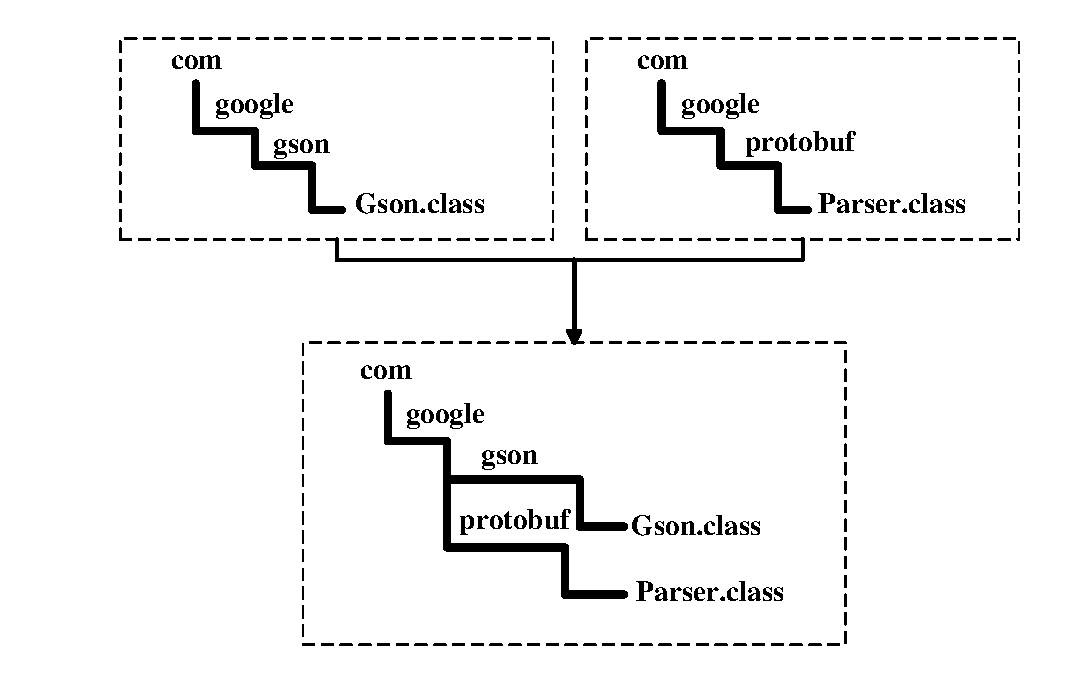
\includegraphics[width=0.9\textwidth]{figure/package.pdf}
	\bicaption[fig:package]{用户代码于库代码文件结构编译前后变化}{用户代码于库代码文件结构编译前后变化}{Fig}{File Hierarchy Change of Android Build Process}
\end{figure}


图~\ref{fig:pacakge}展示了(com.example)与两个库(com.google.gson和com.google.protobuf)共同编译产生的最终DEX文件逻辑层次结构。

\subsection{指纹提取}

组件分析后,库与组件的关系明确,但还有一个问题是一个库可能有不同的版本。
不同版本的组件可能完全相同,然后类的内容有少量不同。
如果直接认定一个某个库的一个组件都有问题,会误杀同一个库的所有不同版本。
为了解决这个问题,我们设计了进一步的“指纹提取”方法,用来区分同一个组件的不同版本,从而能够精确定位到某一个版本的库的组件有隐私问题。

已有的区分一个组件不同版本的方法,通常是构建组件的函数调用关系图,从图的相似性着手来确定不同版本。
然而这个方法在AppShield应用场景内效率过低,从而我们需要设计近似方法,快速区分版本。

我们的方式是对组件的类文件内容进行快速哈希,提取指纹。
通过采用冲突率较低的哈希算法,可以快速断定同一个组件的两个文件是否内容相同(冲突情况为内容不同却误报相同哈希值,可以通过使用适当算法消除)。
内容相同的类可以准确断定是完全相同的,如果两个样本组件是同一个组件同一个版本,则类数量应该相同,并且每一个类的哈希值都应该有对应。
如果这两个条件不满足,则可以断定虽然是同一组件,但是是不同版本。
在实际实现中,我们对产生的Java类文件(.smali文件)进行了SHA-1哈希。
因为SHA-1哈希的冲突率低,而且有硬件优化的实现版本,而且多个类文件可以并行进行哈希,性能好,最后对获得的哈希值表进行排序比较。

\section{相似度分析}
\label{sec:appshield:sim-analysis}

在本节中,我们将介绍一种应用相似度分析的方法,在AppShield中,第三方库和克隆应用的检测都是基于此方法进行。

我们方法的工作流主要由两部分组成,指纹生成和指纹比对。

首先我们会生成一个应用的指纹。
之后我们通过生成的指纹来比较两个应用的相似组件。
与深度组件分析中的指纹提取不同的是,在相似度分析中,需要处理混淆应用。
由于混淆的存在,应用在混下前后的代码会发生改变,所以简单的对代码文件进行哈希来充当指纹在混淆技术下是不可用的。
这里的指纹是需要通过代码的稳定特性生成的,稳定特性是指在代码混淆前后不会发生改变或者改变概率较低的特性。

在指纹比对过程,我们会根据之前生成的指纹,结合应用代码中包的信息,来进行比对算法。
最后我们会报告比对的两个应用有多少包是相似的,有多少类是相似的,以及相似的包和类的具体信息。

接下来我们将先分析总结常用Android混淆器ProGuard的相关功能与配置,并针对ProGuard进行相似度分析。

\subsection{ProGuard}
\label{sec:appshield:proguard}

为了解决混淆,我们需要知道在混淆前后,应用代码有哪些是变化的,哪些是不变的,最终把不变的部分提取出来作为指纹。
因此我们先对目前最常用的Android混淆器ProGuard~\supercite{proguard}进行了研究。
ProGuard是一个Java应用的混淆器,同时也被运用于安卓应用开发过程中。
在安卓开发的官方IDE Android Studio中,已经整合了ProGuard作为安卓开发的混淆器。
ProGuard的输入为应用的jar包,第三方库的jar包,以及ProGuard的配置文件。
ProGuard会根据配置对输入的jar包进行处理,最后将结果写入输出的jar包。
ProGuard的配置会指定混淆时要使用哪些混淆技术,同时还会根据“keep”规则来指定对哪些包、类或者方法不做处理。

\begin{figure}
	\centering
	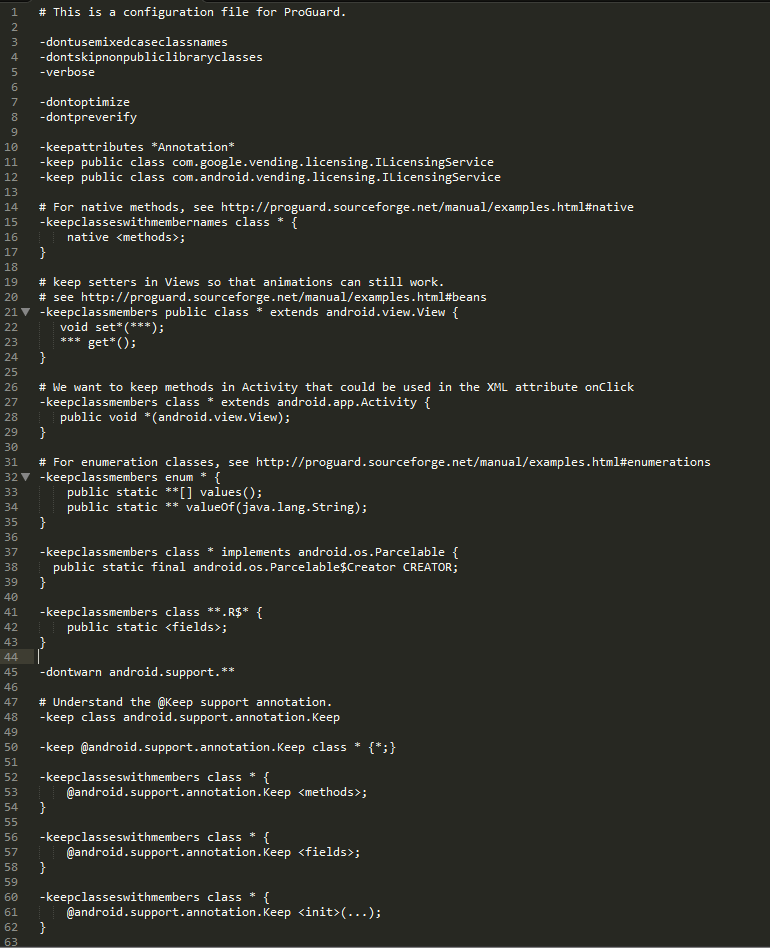
\includegraphics[width=1\textwidth]{figure/proguard-conf.png}
	\bicaption[fig:proguard-conf]{ProGuard Android配置样例}{ProGuard Android配置样例}{Fig}{Example of ProGuard Configuration for Android}
\end{figure}

图~\ref{fig:proguard-conf}为Android构建工具中使用的默认ProGuard配置。
而之前的混淆检测正是利用这份配置,可以看到在ProGuard默认配置中,只对资源类R的public static值域进行了保留,而在应用自身包内一定会存在R。
所以可以利用这一点来进行混淆检测,如果在应用对应包中没有发现R class,则将该应用认定为混淆应用。
这种快速简单的检测方式能够对绝大多数的混淆应用有效。

ProGuard的主要目标是让应用变得更小,同时使得应用的逆向工程变得更加困难。
表~\ref{tab:proguard-obs}展示了在ProGuard中用到的混淆技术,以及对应的配置设置。

\begin{table}[!hpb]
	\centering
	\bicaption[tab:proguard-obs]{ProGuard中不同混淆技术在Android构建中的配置开关}{ProGuard中不同混淆技术的配置开关}{Table}{ProGuard Configuration of 	Different Obfuscation Technique}
	\begin{tabularx}{\textwidth}{|X|c|c|c|X|X}
		\hline
		混淆技术 & 是否默认开启 & 配置开关 & 影响实体\\
		\hline
		标识符重命名 & \cmark & -dontobfuscate (关闭) & 包、类、方法\\
		\hline
		代码缩减 & \cmark & -dontshrink (关闭) & 包、类、方法\\
		\hline
		包结构平坦化 & \xmark & -flattenpackagehierarchy [package\_name] & 包\\
		\hline
		重打包类 & \xmark & -repackageclasses [package\_name] & 类\\
		\hline
		字节码优化 & \xmark & -dontoptimization & 类、方法\\
		\hline
	\end{tabularx}\\
\end{table}

在ProGuard中有两种包结构重组织的方法一种是包平坦化,一种是重打包类。
在进行包结构平坦化时,会将在混淆范围内的包重新组织到一个新的包中,包名为指定的package\_name,默认在根目录下;
而进行重打包类时,会将所有在混淆范围内的类重新打包到一个新包下,包名为指定的pacakge\_name,默认为根目录。
值得注意的是,包结构平坦化保留了一定程度的包结构信息,只是可能会去除掉子包的结构信息,而重打包类是完全去除了包的结构信息与子包的结构信息。

接下来,我们会根据上述总结的ProGuard规则设计我们相似度算法中指纹生成与指纹比对的方法。

\subsubsection{指纹生成}

在Java代码中,类是一个基础单元。
一个类包含着丰富的信息,包括所属包、父类、类的修饰符、成员变量、成员函数等等。
所以我们使用类为单元来进行指纹提取。
我们通过对类的稳定特性进行哈希来生成一个类的指纹。

而如何选择稳定特性是指纹生成的关键,也是相似度检测效果的关键。
由于混淆工具种类繁多,混淆技术花样百出,导致无法做到保证提取出的稳定特性在混淆前后保持不变。
并且即便存在不变的特性,这些特性包含的信息太少,造成太多的信息丢失,以至于在比对时会发生太多的误报,即原本不相似的两个类检测出相似度很高。
所以我们需要在其中找到权衡,在能保证在大多数混淆技术下能够稳定的前提下,要尽可能多的保留代码的信息,从而降低误报,使得相似度检测可用。

在本文所提出的方法中,我们使用的类的稳定特性包括三部分:成员函数,成员变量以及类的元信息。

\begin{itemize}
	\item \textbf{成员函数:} 一个成员函数由三部分组成,函数的修饰符、函数的签名以及函数的字节码。
		首先,函数的字节码在优化和混淆时会发生改变,例如死代码移除和随机化控制流等。
		并且由于混淆过程中会重命名标识符,所以稳定特性不能依赖于任何非Java核心类或者安卓框架类的类名和成员方法名,以及变量名。
		所以我们将这些易变的名字进行了一定程度的模糊处理,对于上述的名字,我们将会使用Object来代替。
		另外,当内联优化操作时,可能会将一个公共的getter内联,这可能就会把公共getter中使用到的私有变量更改成公共变量。
		在ProGuard中,如果allowaccessmodification和优化开启时,ProGuard会对代码进行内联优化,在此优化中,一个方法的access修饰符可能会被拓宽。
		因此我们应该将access修饰符从稳定特性中移除。
		综上所述,一个成员函数的稳定特性由模糊处理后的函数参数类型,函数返回类型,以及部分函数修饰符构成。
	\item \textbf{成员变量:} 一个成员变量由三部分组成,变量的修饰符、变量的类型以及变量的名字。
		由于标识符重命名以及内联优化,我们不能依赖于变量的名字以及access修饰符。
		所以成员变量的稳定特性由模糊处理后的变量类型和部分变量修饰符组成。
	\item \textbf{类元信息:}除了成员函数与变量之外,还有一些额外的信息可以选进类的稳定特性。
		当声明一个类,需要声明类的修饰符、类的父类以及实现的接口。
		在ProGuard中,如果allowaccessmodification和repacakgeclasses开启时,混淆器会将所有重命名过的类重新打包到一个特定的包中。
		因此被重新打包的类的access修饰符可能在重打包过程中被修改。
		因此类的access修饰符不应该被包含在类的稳定特性中。
		最终一个类元信息的稳定特性由模糊处理后的父类类型以及模糊处理后的实现的接口类型。
\end{itemize}

在提取出一个类的所有稳定特性之后,我们需要生成这个类的指纹信息。
我们通过对以上稳定特性分别哈希,得出三个哈希值的列表,分别为成员函数的稳定特性哈希值列表、成员变量的稳定特性哈希值列表以及类元信息的稳定特性哈希值列表。

\subsection{指纹比对}

在比对过程中,有些研究的做法是将类的所有模糊处理后的成员函数签名排序后进行哈希,最后通过比对两个类的哈希值是否相同来判断两个类是否一样。
由于代码缩减的存在,一个类在经过混淆之后,未使用过的成员方法或者成员变量可能会被剔除。
所以一个类在混淆前后的指纹是会发生改变的,其中元信息指纹不会改变,成员变量和成员函数的指纹列表可能会有所缩减。
因此上述方法在处理混淆应用时可能存在问题,导致漏报率增加。

一对同源类A和B存在三种关系:

\begin{enumerate}
	\item A为初始类,经过混淆后变成了B。此时A的成员变量和成员函数指纹列表是B的超集;
	\item A为初始类,经过混淆后变成了B。此时A的成员变量和成员函数指纹列表是B的超集;
	\item A,B都为未混淆类C混淆处理后的类。此时A和B的成员变量和成员	函数指纹信息列表会有相同的指纹元素,也会因为剔除的方法和变量不同而产生差异。
\end{enumerate}

在比对算法中,我们使用了严格相似的标准,即只有出现了上述情况中的前两种我们才会标记类B相似于类A或者类A相似于类B。
在实现中,对于两个类A和B:

\begin{enumerate}
	\item 判断A和B的元信息指纹是否相同;
	\item 判断成员变量指纹列表和成员函数指纹列表是否存在包含关系,如果A包含B,那么标记B相似于A,反之则标记B相似于A,如果A与B一样,则同时标记A相似于B以及B相似于A。
\end{enumerate}

% 由于同构的类经常出现,例如属于Android v4 support library(相同包)的\texttt{SlidingPaneLayout\$SavedState\$1}和\texttt{DrawerLayout\$SavedState\$1},以及Android v4 support library 的\texttt{SlidingPaneLayout\$SavedState\$1}和Android v7 support library的\texttt{Toolbar\$SavedState\$1}(不同包)。
另外,由于代码缩减技术的存在,很多本身不同构的类去除掉没有用掉的成员变量和函数之后,可能会形成同构的情况。
同构类导致类的指纹不是唯一的,所以两个应用的相同指纹的类多并不能代表这两个应用相似。
在这种情况下,就需要引入包的信息来减少同构类造成的误报。

Java中,包的作用是组织类,一个包中包含一组类或接口,这些类和接口功能相关,所以组织在一个包中方便类的查找和使用。
另外包也决定了类的命名空间,包采用树形的存储方式,在一个包中的类的名字不能相同,但是在不同包中的类,名字可以相同。
同时包也规定了包中类的访问权限,以便于更稳定的组织。

由于是文件夹的组织形式,一个包可能包含子包,即子包在母包文件夹下。
这种包之间的关系可能会由于混淆中的包结构重组织而改变,有可能混淆前B是A的子包,而在混淆后B可能已经存在于另外一个包中了。
所以在我们的指纹比对算法中,不会考虑包之间的包含关系。


最后对于一对包A和B,我们会计算出两个相似度\emph{Sim$_{AB}$}和\emph{Sim$_{BA}$}:
\begin{equation}
	\emph{Sim$_{AB}$} = \frac{|\emph{Class$_{AB}$}|}{|\emph{Class$_{A}$}|}.
\end{equation}

\begin{equation}
	\emph{Sim$_{AB}$} = \frac{|\emph{Class$_{AB}$}|}{|\emph{Class$_{A}$}|}.
\end{equation}

其中\emph{Class$_{BA}$}为包B中与包A中相似的类的集合,\emph{Class$_{AB}$}为包A中与包B中相似的类的集合。
而\emph{Class$_{A}$}和\emph{Class$_{B}$}分别表示A和B中类的集合。
当\emph{Sim$_{AB}$}或者\emph{Sim$_{BA}$}超过设置的阈值时,我们会判断A相似于B或者B相似于A。

\subsection{第三方库检测}

AppShield中的第三方库检测基于上文所介绍的相似度检测方法。
我们会收集需要检测的第三方库的不同版本SDK,并对其进行指纹提取。
在实现上,我们先将第三方库的SDK jar包使用Android构建工具dx打包成APK,之后就能使用之前提到的相似度检测的方法。
我们将要检测的应用的指纹与所有版本的SDK指纹一一比对,比如对于一个应用A和n个版本的第三方库B$_{1}$ - B$_{n}$,如果发现任意一个版本的B$_{i}$,\emph{Sim$_{B_{i}A}$}超过了0.7,那么我们就判断应用A包含第三方库B。

\subsection{克隆应用检测}

AppShield中的克隆应用检测同样也是基于相似度检测的方法。
由于在克隆应用中,只会重打包很少一部分信息,所以互相的相似度都应该要求在一个很高的水平上,并不会出现克隆应用A和B,A相似与B而B不相似于A。
所以在实现上我们将相似度比对的阈值设置在了0.9,并且需要\emph{Sim$_{AB}$}和\emph{Sim$_{BA}$}同时超过了阈值,我们才将这对应用标记为潜在的克隆应用。

\section{本章小结}
\label{sec:appshield:conclusion}

本章对AppShield的设计与实现做了详细的介绍。
首先介绍了AppShield大致架构,其次对应用文件来源进行了阐述,之后对问题组件分析模块进行了描述,最后对AppShield中第三方库检测和克隆应用检测用到的相似度分析方法进行了介绍。